% Chapitre 15 -- ED-24 : reconstruction indépendante, rejeu par le noyau et audit du corpus openai/NavierStokesAndEuler
% Sources : results/discovery_journal_2026/TOP20.json (pick 15), papers/p2_navier_stokes_audit/{main.tex,AUDIT.md,REVISION.md,publication_meta.json}.
% Figure : code/fig15.py.
\chapter[Remonter la machine des autres]{Remonter la machine des autres dans son propre atelier}

\reference{Publié le 26 octobre 2026. doi:10.5281/zenodo.23661381}

\section*{L'idée en une image}

Les équations de Navier--Stokes décrivent l'écoulement des fluides, de l'eau dans un tuyau à
l'air autour d'une aile. L'Institut Clay a fait d'une question à leur sujet l'un de ses
\og problèmes du millénaire\fg{} : les solutions lisses existent-elles toujours, ou peuvent-elles
\og casser\fg{} ? Sa description officielle propose quatre énoncés possibles ; deux d'entre eux
affirment une rupture.

En 2026, OpenAI a publié un ensemble de fichiers Lean, appelé ici \emph{le corpus}, dont les
auteurs présentent le contenu comme la formalisation de deux de ces énoncés de rupture, plus une
singularité pour les équations d'Euler, une autre description des fluides, qui ne figure pas sur la
liste du Clay. \textbf{Le mérite de
ces preuves revient aux auteurs du corpus.} Le travail raconté ici n'en a écrit aucune ligne : il
les a contrôlées de l'extérieur. \textbf{Ce n'est pas l'annonce qu'un problème du Clay est
résolu} ; seul l'Institut Clay, par sa propre procédure, peut en décider.

\begin{analogie}
On reçoit les plans d'une machine célèbre. On la remonte pièce par pièce dans son propre atelier
pour voir si elle tourne, sans prétendre l'avoir inventée. \emph{Où l'image s'arrête :}
\og tourner\fg{} veut dire ici que chaque étape logique est acceptée par le juge de Lean, pas que
la machine fait exactement ce que demande le problème du prix ; cela se juge en lisant. Et
l'atelier n'est pas entièrement le nôtre : le juge est le même que celui des auteurs, et la
grande bibliothèque mathématique utilisée a été reprise, pas revérifiée.
\end{analogie}

\section*{Ce qui a été fait}

Les 2\,440 modules du corpus ont été recompilés à partir des sources, avec la version exacte des
outils choisie par les auteurs : aucune erreur, aucun avertissement dans les parties prouvées.
Les quatre théorèmes principaux ne reposent que sur les trois axiomes de la liste courte. Des
balayages du texte et de l'environnement n'ont trouvé aucun moyen détourné de contourner le juge,
et chaque balayage a bien attrapé les pièges plantés exprès pour le tester.

Puis vient l'étape décisive : le \emph{rejeu}. On renvoie au noyau de Lean chacune des
déclarations stockées, pour qu'il revérifie que chaque preuve établit bien ce que son étiquette
affirme. 88\,400 déclarations lui ont été envoyées : 53\,752 pour Navier--Stokes et 34\,648 pour
Euler. Réponse : \og REPLAY OK\fg{} dans les deux cas. Par conception, l'outil saute 51 petites
pièces générées automatiquement par le compilateur (12 et 39), dont aucune n'entre dans une
preuve, et 4 doublons identiques. Enfin, les énoncés prouvés ont été comparés aux énoncés de
référence fournis avec le corpus : ils sont identiques (au nom près de quelques variables internes), et une version volontairement altérée de
la référence est bien détectée.

\begin{encadre}
\textbf{À faire avec un crayon : pourquoi la liste des axiomes ne suffit pas.} Avec un réglage spécial, on peut
ranger dans un fichier une déclaration que le juge n'a jamais regardée. Le contrôle planté par
l'auditeur porte l'étiquette \og $2=3$\fg{}, et sa \og preuve\fg{} est simplement \og $2$ est égal
à lui-même\fg{}. Demandez la liste de ses axiomes : la preuve n'en cite aucun, elle passe.
Demandez au juge de rejouer la déclaration : il compare ce que la preuve établit, $2=2$, avec ce
que l'étiquette réclame, $2=3$, et refuse. C'est pour cela que le rejeu complet a été fait. Les
comptes se vérifient aussi au crayon : $53\,752+34\,648=88\,400$ et $12+39=51$.
\end{encadre}

\section*{Comment on s'est assuré que ce n'est pas faux}

Les quatre théorèmes sont \niveau{A} \emph{Le juge a regardé} : vérifiés par le noyau, axiomes dans
la liste courte, et rejoués en entier ; tout cela a été refait dans cette étude. La fidélité des énoncés est \niveau{C} : une lecture comparée avec la description
officielle, faite ici par des agents d'IA et non par un humain, sans vérification à la machine. Elle conclut que l'énoncé Lean de la première rupture,
sur l'espace entier, est fidèle ; pour la seconde, sur un domaine périodique, elle est fidèle à
la description corrigée par ses errata, avec une réserve : la condition ajoutée sur la pression
rend l'affirmation Lean plus faible qu'une lecture du seul texte principal. Cette lecture, écrite
sans voir un audit antérieur, est d'accord avec lui sur chaque ligne.

Un agent auditeur distinct a tout refait avec ses propres scripts : son propre rejeu (les deux
fermetures passent, la fausse déclaration est rejetée), sa propre liste d'axiomes, une
vérification par le juge que les énoncés de référence se déduisent mot pour mot des théorèmes du
corpus (quatre versions altérées échouent), et la preuve que les classes de solutions ne sont pas
vides. Il n'a trouvé ni brèche, ni énoncé faux, ni nombre faux. Son verdict, \og accepter avec
corrections\fg{}, demandait deux corrections de formulation : une phrase invitait à conclure plus
que le texte ne l'autorise, et \og toutes les déclarations passent le juge\fg{} n'était pas exact
à la lettre, à cause des pièces sautées. Les deux sont corrigées. Aucun humain n'a relu ce
travail.

\section*{Ce que ça ne dit pas}

\begin{limite}
\begin{itemize}
\item \textbf{Aucun problème du Clay n'est déclaré résolu.} La conclusion est conditionnelle : si
  l'énoncé Lean traduit fidèlement la description officielle, et si Lean et sa bibliothèque sont
  sains, l'objet formel prouve l'énoncé de rupture visé. Ce n'est pas une décision du Clay.
\item Un seul juge, conduit par deux programmes ; aucun second juge indépendant n'a été lancé, et
  la vérification complète de la bibliothèque depuis zéro non plus.
\item La bibliothèque mathématique a été reprise telle quelle, pas revérifiée.
\item Les mathématiques de la preuve n'ont pas été relues par des personnes, et les articles des
  auteurs n'ont pas été lus.
\end{itemize}
\end{limite}

\section*{Pour aller plus loin}

Le papier (11 pages, en anglais), qui explique pas à pas le mécanisme de la fausse déclaration :
doi:10.5281/\allowbreak zenodo.23661381. Le corpus lui-même : github.com/openai/NavierStokesAndEuler.

\begin{figure}[ht]
\centering
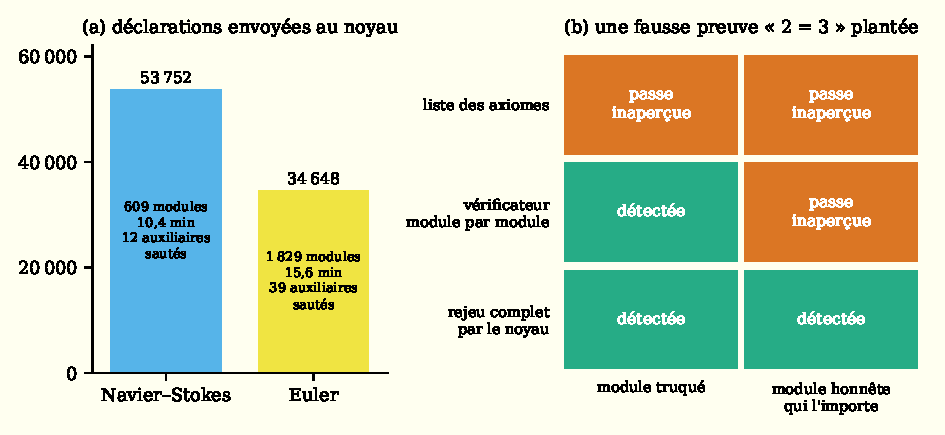
\includegraphics[width=\linewidth]{figures/c15_rejeu}
\caption{(a) Déclarations renvoyées au noyau, par corpus. (b) Seul le rejeu complet attrape la fausse preuve, y compris chez un module honnête qui l'importe.}
\end{figure}
